\documentclass{article}
\renewcommand{\rmdefault}{psbx}
\usepackage[utf8]{inputenc}
\usepackage[T1]{fontenc}
\usepackage{textcomp}
\usepackage{eulervm}
\usepackage{amsmath}
\usepackage{amssymb}

\setlength{\textwidth}{160mm}
\setlength{\oddsidemargin}{0mm}
\setlength{\parindent}{0 mm}

\newcommand{\bfa}{{\bf a}}
\newcommand{\bfb}{{\bf b}}
\newcommand{\bfm}{{\bf m}}
\newcommand{\bfs}{{\bf s}}
\newcommand{\bfz}{{\bf z}}
\newcommand{\E}{{\mathbb E}}
\newcommand{\V}{{\mathbb V}}

\usepackage{tikz}
\usetikzlibrary{arrows,shapes,backgrounds,patterns,fadings,decorations.pathreplacing,decorations.pathmorphing}
\tikzset{>=stealth'}

\title{The Cart and Pole Task}
\author{Carl Edward Rasmussen}
\date{July 3rd 2014}

\begin{document}

\maketitle
\begin{center}
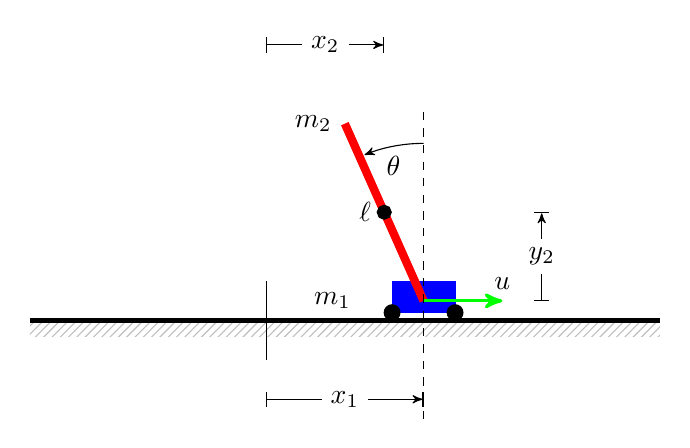
\begin{tikzpicture}
\def\xcart {2}     % x-position of center of the cart
\def\ycart {0.25}  % y-position of center of the cart
\def\wheelR {0.1} % Radius of wheels
\def\cartW  {0.8} % Width of the cart
\def\cartH {0.4}  % Heigt of the cart
\def\ang {22}     % Angle theta
\def\xtipR {-1}   % Relative x-Position of tip of the pendululum with respect to center of cart
\def\ytipR {2.25} % Relative x-Position of tip of the pendululum with respect to center of cart
% rail:
  \draw[draw=none,pattern=north east lines,pattern color=lightgray](-3,0) rectangle (5,-0.2);
  \draw[draw=black,ultra thick] (-3,0) -- (5,0);
 % cart:
 \draw[draw=blue,fill=blue] (\xcart-\cartW/2,\wheelR) rectangle (\xcart+\cartW/2,\wheelR+\cartH);  
 \draw[draw=black,fill=black] (\xcart-\cartW/2,\wheelR) circle (\wheelR cm);
 \draw[draw=black,fill=black] (\xcart+\cartW/2,\wheelR) circle (\wheelR cm);
 \node[anchor=east] at (\xcart-\cartW,\ycart) {$m_1$};
% pole:
 \draw[draw=red, line width = 3pt] (\xcart,\ycart) -- (\xcart+\xtipR,\ycart+\ytipR)node[anchor= east] {$m_2$}  node[anchor= east, midway]  {$\ell$};
  \draw[draw=black, line width = 3pt] (\xcart+\xtipR/2,\ycart+\ytipR/2) circle (0.04cm);
%% geometry:
 \draw[draw=black, dashed] (\xcart,\ycart-1.5) -- (\xcart,\ycart+2.5);
 \draw[draw=black] (0,-.5) -- (0,.5);
 \draw [->] ([shift=(90:2)]\xcart,\ycart)  arc (90:90+\ang:2) node[anchor =north, midway] {$\theta$};;
 \draw [|->|,draw=black] (0,-1) -- (\xcart,-1) node[fill=white, midway] {$x_1$};
 \draw[|->|,draw=black] (\xcart+\xtipR+2.5,\ycart) -- (\xcart+\xtipR+2.5,\ycart+\ytipR/2) node[fill=white, midway]  {$y_2$};
 \draw[|->|,draw=black] (0,\ycart+\ytipR+1) -- (\xcart+ \xtipR/2,\ycart+\ytipR+1) node[fill=white, midway]  {$x_2$};
% 
%% force:
 \draw[very thick,draw=green,->]  (\xcart,\ycart) -- (\xcart +1,\ycart) node[anchor=south]  {$u$};

\end{tikzpicture}  
\end{center}

The cart and pole dynamical system consists of a cart (mass $m_1$) and
an attached pedulum (mass $m_2$, length $\ell$) which swings freely in
the plane. The pendulum angle, $\theta$, is measured anti-clockwise
from hanging down (diagram would be useful). The cart can move
horizontally, with an applied external force $u$, and coefficient of
friction $r$. Typical values are: $m_1=0.5{\rm kg}$, $m_2=0.5{\rm
  kg}$, $\ell=0.6{\rm m}$ and $r=0.1{\rm N/m/s}$.

The coordinates $x_2$ and $y_2$ of the midpoint of the pendulum are
\[
x_2\;=\;x_1-\tfrac{1}{2}\ell\sin\theta,\qquad
y_2\;=\;\tfrac{1}{2}\ell\cos\theta,
\]
and the squared velocity of the cart and the midpoint of the pendulum are
\[
v_1^2\;=\;\dot x_1^2,\qquad v_2^2\;=\;\dot x_2^2+\dot y_2^2\;=\;
\dot x_1^2+\tfrac{1}{4}\ell^2\dot\theta^2-\ell\dot x_1\dot\theta\cos\theta.
\]
The system Lagrangian is
\[
\begin{split}
L\;=\;T-V\;=\;
\tfrac{1}{2}m_1v_1^2+\tfrac{1}{2}m_2v_2^2+\tfrac{1}{2}I\dot\theta^2-m_2gy_2
\;\Rightarrow\\
\protect\boxed{L\;=\;\tfrac{1}{2}(m_1+m_2)\dot
x_1^2+\tfrac{1}{6}m_2\ell^2\dot\theta^2-\tfrac{1}{2}m_2\ell(\dot
x_1\dot\theta+g)\cos\theta}
\end{split}
\]
where we have used the angular moment of inertia around the pendulum
midpoint is $I=\tfrac{1}{12}m\ell^2$, and $g=9.82 {\rm m/s^2}$ is the
accelleration of gravity.

The equations of motion are
\[
\frac{d}{dt}\frac{\partial L}{\partial\dot q_i}-\frac{\partial
  L}{\partial q_i}\;=\;Q_i,
\]
where $Q_i$ are the non-conservative forces. In our case
\begin{alignat}{3}
\frac{\partial L}{\partial\dot x_1}\;&=
\;(m_1+m_2)\dot x_1-\tfrac{1}{2}m_2\ell\dot\theta\cos\theta,&\qquad
\frac{\partial L}{\partial x_1}\;&=\;0,\\
\frac{\partial L}{\partial\dot\theta}\;&=\;\tfrac{1}{3}m_2\ell^2\dot\theta
-\tfrac{1}{2}m_2\ell\dot x_1\cos\theta,&\qquad
\frac{\partial L}{\partial\theta}\;&=\;\tfrac{1}{2}m_2\ell(\dot
x_1\dot\theta+g)\sin\theta,
\end{alignat}
leading to the equations of motion
\[
\boxed{
(m_1+m_2)\ddot x_1-\tfrac{1}{2}m_2\ell\ddot\theta\cos\theta
+\tfrac{1}2m_2\ell\dot\theta^2\sin\theta\;=\;u-r\dot x_1,\qquad
2\ell\ddot\theta-3\ddot x_1\cos\theta-3g\sin\theta\;=\;0.}
\]
Collecting the four variables $\bfz=(x_1,\theta,\dot x_1, \dot\theta)$
the equations of motion can be conveniently expressed as four coupled
differential equations
\[
\frac{d\bfz}{dt}\;=\;\left\{\begin{array}{l}z_3\\ z_4\\[1em]
\displaystyle \frac{-2m_2\ell z_4^2\sin z_2+3m_2g\sin z_2\cos z_2+4u-4rz_3}
{4(m_1+m_2)-3m_2\cos^2 z_2}\\[1em] \displaystyle
\frac{-3m_2\ell z_4^2\sin z_2\cos z_2+6(m_1+m_2)g\sin z_2+6(u-rz_3)\cos z_2}
{4\ell(m_1+m_2)-3m_2\ell\cos^2 z_2}, \end{array}\right.
\]
which can be simulated numerically.

\subsection*{Linearized Dynamics}

Linearizing the dynamics around the goal state, we can write the
following approximation
\[
\frac{d\bfz}{dt}\;\simeq\;q^{-1}(A\bfz+B u),\qquad
A\;=\;\begin{bmatrix}
0&0&q&0\\
0&0&0&q\\
0&3\ell m_2g&-4\ell r&0\\
0&6(m_1+m_2)g&-6r&0 \end{bmatrix},\qquad
B\;=\; \begin{bmatrix}
0\\ 0 \\ 4\ell \\ 6\end{bmatrix}
\]
where $q = \ell(4m_1+m_2)$.

\subsection*{Loss Function}

The instantaneous loss is given by
\[
F\;=\;1-\exp(-\frac{d^2}{2a^2}),
\]
were $d^2$ is the squared distance between the tip of the pendulum and
the point at distance $\ell$ above the origin, and $a$ is the
\emph{width} parameter. Note that the instantaneous loss does not
depend on the speed variables, $\dot x_1$ and $\dot\theta$. The
squared distance is
\[
d^2\;=\;x^2+(\ell-y)^2\;=\;(x_1-\ell\sin\theta)^2+(\ell-\ell\cos\theta)^2
\;=\;(\tilde\bfz-\mu)^\top Q(\tilde\bfz-\mu),
\]
where $\tilde\bfz$ is $\bfz$ augmented by two coordinates $\sin\theta$ and
$\cos\theta$ and
\[
Q\;=\;C^\top C,\qquad
C\;=\;\begin{bmatrix}1&0&0&0&-\ell&0\\ 0&0&0&0&0&\ell\end{bmatrix},\qquad
\mu\;=\;\begin{bmatrix}0&0&0&0&0&1\end{bmatrix}^\top.
\]
The \emph{expected loss}, averaging over the possibly uncertain states
is therefore
\[
\E[F(\tilde\bfz)]\;=\;1-\int F(\tilde\bfz)p(\tilde\bfz)d\tilde\bfz,
\]
which can be evaluated in closed form for Gaussian $p(\tilde\bfz)$, see
reward.pdf. Since the augmented state $\tilde\bfz$ will not generally
be Gaussian even if $\bfz$ is Gaussian, we project on to the closest
Gaussian by matching first and second moments.
\end{document}

